%
% Documento: Estrutura
%

\chapter{ESTRUTURA}

A estrutura de acordo com a NBR-14724, compreende tr\^{e}s elementos: pr\'{e}-textuais, tex-tuais e p\'{o}s-textuais.

\begin{figure}[H]
	\vspace*{0,2cm}
    \centering
    \caption{Ilustra\c{c}ão da estrutura}
    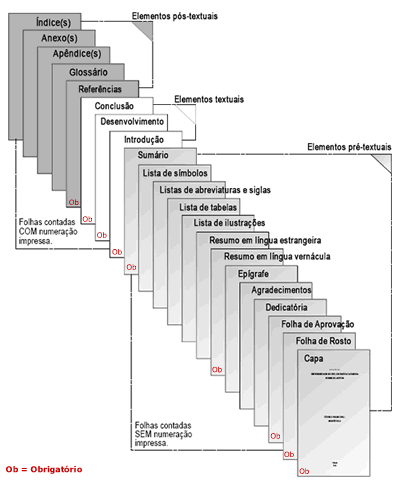
\includegraphics[width=0.6\textwidth]{./04-figuras/abnt}
    \label{fig:ilustfig2}
\end{figure}
\vspace*{-0,9cm}
{\raggedright \fonte{Disponível em: <https://www.intelligentsia.zip.net/estruturamonografia>. Acesso em: 15 ago. 2014.}}\\

Os elementos pr\'{e}-textuais são compostos de estruturas
obrigat\'{o}rias: Capa, Folha de ros-to, Folha de aprova\c{c}ão e Sumário. E estruturas opcionais: Lombada, Errata, Dedicat\'{o}ria, Agra-decimentos, Epígrafe, Resumo na língua vernácula, Resumo em língua estrangeira, Lista de ilustra\c{c}ões, Lista de abreviaturas e siglas e Lista de símbolos.

Os elementos textuais são compostos de Introdu\c{c}ão,
Desenvolvimento e Conclusão. Os elementos p\'{o}s-textuais podem \'{e} obrigat\'{o}rios usar as Refer\^{e}ncias.  E são elementos opcionais: Glossário, Ap\^{e}ndice, Anexo e Índice.

\section{ELEMENTOS PR\'{e}-TEXTUAIS}

\subsection{Capa}

Elemento obrigat\'{o}rio, sobre o qual se imprimem as informa\c{c}ões
indispensáveis \`{a} indica-\c{c}ão do trabalho, na seguinte ordem: nome completo do aluno, título do trabalho, subtítulo se houver, cidade da institui\c{c}ão onde o documento deve ser apresentado, ano de dep\'{o}sito (data da entrega).

\subsection{Lombada}

Elemento opcional, onde as informa\c{c}ões devem ser impressas
conforme a norma NBR 12225: nome do autor, impresso longitudinalmente e legível do alto para o p\'{e} da lombada. Esta forma possibilita a leitura quando o trabalho está no sentido horizontal, com a face voltada para cima; título do trabalho, impresso da mesma forma que o nome do autor. Elementos alfanum\'{e}ri-cos de identifica\c{c}ão, por exemplo: v. 3.

\subsection{Folha de Rosto}

O anverso da folha de rosto deve conter os elementos na seguinte
ordem: nome completo do aluno, título do trabalho, subtítulo se houver, natureza do trabalho e objetivo (grau pretendi-do), nome da institui\c{c}ão a que \'{e} submetido, área de concentra\c{c}ão, nome do orientador, local da institui\c{c}ão onde deve ser apresentado, ano de entrega.

\subsection{Errata}

A errata consiste em uma lista das folhas e linhas em que ocorrem
erros, seguida das de-vidas corre\c{c}ões. Deve ser inserida ap\'{o}s a folha de rosto.

\subsection{Folha de aprova\c{c}ão}

Elemento obrigat\'{o}rio, a folha de aprova\c{c}ão deve conter: nome do
autor, título por exten-so, subtítulo, local e data de aprova\c{c}ão, nome, assinatura e institui\c{c}ão dos membros componen-tes da banca examinadora.

\subsection{Dedicat\'{o}ria}

Folha opcional, onde o aluno presta homenagem ou dedica seu trabalho.

\subsection{Agradecimentos}

Folha opcional, dirigida \`{a}queles que contribuíram para a
elabora\c{c}ão do trabalho.

\subsection{Epígrafe}

Elemento opcional, onde o aluno apresenta uma cita\c{c}ão, seguida da
indica\c{c}ão de autoria, relacionada com a mat\'{e}ria tratada no corpo do trabalho. As epígrafes tamb\'{e}m podem ser apre-sentadas nas folhas de abertura das se\c{c}ões primárias.

\subsection{Resumo}

Consiste na apresenta\c{c}ão concisa dos pontos principais de um
texto. Devem ser apresentados, de forma clara, os objetivos, o desenvolvimento e as conclusões. Constitui-se em uma sequ\^{e}ncia de frases objetivas e não uma simples enumera\c{c}ão de t\'{o}picos. Deve ser seguido das palavras representativas do conteúdo do trabalho, isto \'{e}, palavras-chave e/ou descritores.

\subsection{Abstract}

Consiste em uma versão do resumo em idioma de divulga\c{c}ão
internacional. Deve ser se-guido das palavras representativas do conteúdo do trabalho, isto \'{e}, palavras-chave e/ou unitermos, na língua.

\subsection{Lista de ilustra\c{c}ões}

As ilustra\c{c}ões (figuras, quadros, tabelas, gráficos) devem ser
numeradas na ordem em que aparecem no texto. \'{e} recomendável que sejam feitas listas separadas para cada tipo de ilus-tra\c{c}ão. Em cada lista devem constar: número, título e página. Quando as ilustra\c{c}ões forem em grande número e/ou em tamanho maior, podem ser agrupadas no final do trabalho como ap\^{e}n-dice. As ilustra\c{c}ões, com exce\c{c}ão de tabelas, quadros e gráficos, podem ser sinalizadas no texto ou entre par\^{e}nteses no final da frase, com o termo Figura.

\subsection{Lista de abreviatura e siglas}

Consiste na rela\c{c}ão alfab\'{e}tica das abreviaturas e siglas
utilizadas no texto, seguidas das palavras ou expressões correspondentes grafadas por extenso. Recomenda-se a elabora\c{c}ão de lista pr\'{o}pria para cada tipo.

\subsection{Lista de símbolos}

Os símbolos devem ser apresentados na lista na ordem em que
aparecem no texto, com o devido significado.

\subsection{Sumário}

Consiste na enumera\c{c}ão das principais divisões, se\c{c}ões e outras
partes do trabalho, na ordem em que aparecem no texto, acompanhadas da página inicial. As divisões devem estar numeradas em algarismos arábicos, a partir da Introdu\c{c}ão at\'{e} \`{a}s Refer\^{e}ncias. Havendo subdivi-sões, deve ser adotada a numera\c{c}ão progressiva, sempre em número arábico e a distin\c{c}ão de caracteres, de acordo com a NBR-6027.

\section{ELEMENTOS TEXTUAIS}

\subsection{Introdu\c{c}ão}

\'{e} a parte inicial do texto onde devem constar a delimita\c{c}ão do
assunto tratado, os objeti-vos da pesquisa e os outros elementos necessários para situar o tema do trabalho.

\subsection{Desenvolvimento}

Parte do texto que cont\'{e}m a exposi\c{c}ão ordenada e pormenorizada do
assunto. Divide-se em se\c{c}ões e subse\c{c}ões, que variam em fun\c{c}ão da abordagem do tema e do m\'{e}todo.

\subsection{Conclusão}

Final do texto na qual se apresentam as conclusões correspondentes aos objetivos ou hip\'{o}teses.

\section{ELEMENTOS P\'{o}S-TEXTUAIS}

\subsection{Referencias}

\'{e} o conjunto padronizado de elementos descritivos, retirados de
um documento, que permite a sua identifica\c{c}ão individual. Denomina-se ainda de Refer\^{e}ncias a lista composta de documentos padronizados e utilizados na elabora\c{c}ão de um trabalho acad\^{e}mico.

\subsection{Ap\^{e}ndice}

Consiste em um texto ou um documento elaborado pelo autor, a fim
de complementar sua argumenta\c{c}ão, sem prejuízo da unidade nuclear do trabalho. Os ap\^{e}ndices são identificados por letras maiúsculas consecutivas, travessão e pelos respectivos títulos.

\subsection{Anexo}

Consiste em um texto ou documento não elaborado pelo autor, que
serve de fundamen-ta\c{c}ão, comprova\c{c}ão e ilustra\c{c}ão. Os anexos são identificados por letras maiúsculas consecuti-vas, travessão e pelos respectivos títulos.

\subsection{Índice}

Elemento opcional, elaborado conforme a NBR 6034.

